\chapter{Bandstructure}


\section{LCAO Theory}
Before presenting the more elegant manner in which electronic bandstructure of many-particle systems can be determined via a combination of the principles behind second quantisation formalism and Bloch's theorem, I would like to present the generic (or more bluntly, $obsolete$) technique of analysing bandstructure using the principles of first quantisation. \\

Consider a linear chain of identical hydrogenic atoms ($ns$ orbitals) with individual lattice points separated by a distance $a$. From the LCAO theory, the generalized wavefunction of the system can be expressed as a linear combination of orbitals at the lattice sites:
\begin{equation*}
    \psi = c_{1}\phi_{1} + c_{2}\phi_{2} + c_{3}\phi_{3} + ... = \sum_{n}c_{n}\phi_{n}
\end{equation*}

where $x_{n}$ is the position of the $n$th atom. The atoms, being identical, contribute equally to the LCAO in terms of their wavefunction amplitude but with different phase factors to account for their periodic distribution. More formally, this idea is captured via Bloch's theorem, which presents a generalised wavefunction for particles in a periodic lattice:
\begin{equation*}
    \psi_{k}(\vec{r}) = e^{i\vec{k}\cdot \vec{r}}u_{k}(\vec{r})
\end{equation*}

where $u_{k}(\vec{r})$ is called the \textit{cell function}, and represents atoms in the unit cell. For the toy model described above, the Bloch wavefunction is given by
\begin{equation}
    \psi_{k} = \sum_{n=1}^{N} e^{ikna}\phi_{n}
\end{equation}

The Bloch wavefunction incorporates the real-space symmetry of the lattice into the $k$-space in the sense that for $k > \frac{\pi}{a}$, the wavefunction merely acquires a global phase, and this does not affect the expectation value of measurables. The energy eigenvalue of the Bloch wavefunction serves as a direct measure of the $E-k$ relationship and is given by
\begin{equation}
    E = \frac{\int_{\mathcal{R}} \psi_{k}^{\dagger} \mathcal{H}\psi_{k}\: dx}{\int_{\mathcal{R}} \psi_{k}^{\dagger} \psi_{k}\: dx}
\end{equation}

The expectation value of the Hamiltonian can be simplified as
\begin{equation*}
    \int_{\mathcal{R}} \psi_{k}^{\dagger}\mathcal{H}\psi_{k} \: dx = \sum_{n=1}^{N} \sum_{m=1}^{N}e^{i(n-m)ka} \int_{\mathcal{R}} \phi_{m}^{\dagger}\mathcal{H}\phi_{n} \: dx
\end{equation*}

Applying the constraints of the tight-binding approximation, the integral term involved in RHS can be simplified into three distinct cases: $\alpha$ if $m = n$, i.e., the potential energy corresponding to each lattice site, $\beta$ if $|m-n| =1$, i.e., the lattice sites correspond to nearest neighbours, and $0$ otherwise.

\begin{equation*}
   \begin{aligned}
   	  \int_{\mathcal{R}} \psi_{k}^{\dagger}\mathcal{H}\psi_{k} \: dx &= N(\alpha + \beta[e^{-ika}+e^{ika}]) = N(\alpha + 2\beta \text{cos}(ka)) \\
   	  \int_{\mathcal{R}} \psi_{k}^{\dagger}\psi_{k} \: dx &= \sum_{n=1}^{N} \sum_{m=1}^{N}e^{i(n-m)ka} \int_{\mathcal{R}} \phi_{m}^{\dagger}\phi_{n}\: dx = N
   \end{aligned}
\end{equation*}

since the integral term in the RHS evaluates as null unless $m = n$. Hence, the energy eigenvalue is given by
\begin{equation}
    E_{k} = \alpha + 2\beta \text{cos}(ka)
\end{equation}

As pointed out earlier, for values of $k > \frac{\pi}{a}$, the $E-k$ diagram can be simply folded over into the region bounded by $-\frac{\pi}{a} < k < \frac{\pi}{a}$. This region is otherwise known as the first \textit{Brillouin zone}. \\

\newpage

Next, we add an additional layer of complexity to the simple toy model by considering two atoms (not necessarily identical) per unit cell in a three-dimensional lattice. The trial wavefunction for the same can be expressed as
\begin{equation*} 
    \psi_{k}(\vec{r}) = \frac{1}{\sqrt{N}}\sum_{n=1}^{N}\{c_{1}(k) \: \phi_{1}(\vec{r_{1}}-\vec{R_{n}}-\vec{d_{1}})e^{i\vec{k}\cdot \vec{d_{1}}} + c_{2}(k)\: \phi_{2}(\vec{r_{2}}-\vec{R_{n}}-\vec{d_{2}})e^{i\vec{k}\cdot \vec{d_{2}}}\}
\end{equation*}

where $N$ is the number of unit cells (theoretically tending to a \textit{countable infinity}), and $d_{1}, d_{2}$ represent the displacement of atomic centres 1 and 2 respectively, w.r.t the centre of the unit cell under consideration, which itself is located at $\vec{R}_{n}$. $c_{1}(k), c_{2}(k)$ are the contributions of atomic orbitals 1 and 2, respectively, to the Bloch wavefunction. \\

Denote $\alpha_{1} = \int_{\mathcal{R}} \phi_{1}^{\dagger}\mathcal{H}\phi_{1}\: d^{3}\vec{r}$, $\alpha_{2} = \int_{\mathcal{R}} \phi_{2}^{\dagger}\mathcal{H}\phi_{2}\: d^{3}\vec{r}$, and $\beta = \int_{\mathcal{R}} \phi_{i}^{\dagger}\mathcal{H}\phi_{j}\: d^{3}\vec{r} = \int_{\mathcal{R}} \phi_{j}^{\dagger}\mathcal{H}\phi_{i}\: d^{3}\vec{r}$ (for $|i-j| = 1$). Using the standard Fourier technique for eliminating the integrals yields the following set of equations
\begin{equation*}
    \begin{aligned}
        \alpha_{1} c_{1}(k) + \beta \sum_{n}e^{i\vec{k}\cdot \vec{d}_{nn}} c_{2}(k) &= E(k) c_{1}(k) \\
        \alpha_{2} c_{2}(k) + \beta \sum_{n}e^{-i\vec{k}\cdot \vec{d}_{nn}} c_{1}(k) &= E(k) c_{2}(k)
    \end{aligned}
\end{equation*}

where $d_{nn}$ is the distance between nearest neighbours in the lattice. In matrix form, these equations can be represented as
\begin{gather*}
    \begin{bmatrix}
        \alpha_{1} & \beta g(k) \\ \beta g^{\dagger}(k) & \alpha_{2}
    \end{bmatrix}
    \begin{bmatrix}
        c_{1}(k) \\ c_{2}(k)
    \end{bmatrix}
    = E(k) \:
    \begin{bmatrix}
        c_{1}(k) \\ c_{2}(k)
    \end{bmatrix}
\end{gather*}  

where $g(k) = \sum_{m}e^{i\vec{k}\cdot \vec{d}_{m}}$. Solving for the eigenvalues of the matrix, we obtain, 

\begin{equation}
    E = \frac{\alpha_{1} + \alpha_{2}}{2} \pm \sqrt{\left(\frac{\alpha_{1} - \alpha_{2}}{2}\right)^{2} + \beta^{2}|g(k)|^{2}}
\end{equation}

Under the limit that the atoms in the unit cell are identical, $\alpha_{1} = \alpha_{2} = \alpha$ and are equally spaced at a distance $a$ apart, the energy eigenvalues simplify to $E(k) = \alpha \pm \beta (e^{-ika}+e^{ika}) = \alpha \pm 2\beta \text{cos}(ka)$. If the atoms are non-identical, then the degeneracy of the non-bonding orbital is broken, and there exists a \textit{band gap} in the material. 


\section{Discretizing the Hamiltonian}

While the detailed mathematical analysis outlined in the previous section is useful for gaining a physical intuition of the system, we need to generalize this process to basis sets other than the simple 1-D chain of atoms that we have been working on. In order to do so, we have to discretize the Schrödinger's equation such that we can formulate the Hamiltonian and the corresponding eigenvectors as matrices. This is also useful as a computational tool, since equations need to be discretized in order to run computational simulations. However, its utility is not merely limited as a computational tool- it will be shown that the idea of the wavefunction being a superposition of basis functions is essential to the structure of quantum mechanics in general. \\

Consider, for example, the classical problem of a perticle trapped in a box bounded by infinitely high walls. The Schrödinger's equation governing the system is given by
\begin{equation*}
    -\frac{\hbar^2}{2m}\frac{d^2 \psi}{dx^2} + U_0 \psi = E \psi
\end{equation*} 

The setup can be described as a discrete system, consisting of $N$ lattice sites separated by some infinitesimal lattice constant $a$ such that the ansatz satisfying this equation can be discretized as $\psi_{n} = \psi_{0}e^{ikna}$ via the Bloch's theorem (observe that the basis set is singleton \{$\psi_0$\}). The Hamiltonian can be discretized as follows
\begin{equation*}
\begin{aligned}
    \left.\frac{d\psi}{dx}\right|_{x=n} &= \frac{\psi|_{x=n+\frac{1}{2}}-\psi|_{x=n-\frac{1}{2}}}{a} \\
    \left.\frac{d^2 \psi}{dx^2}\right|_{x=n} &= \frac{\frac{d\psi}{dx}|_{x=n+\frac{1}{2}}-\frac{d\psi}{dx}|_{x=n-\frac{1}{2}}}{a} = \frac{\psi_{n+1}-2\psi_{n}+\psi_{n-1}}{a^2}
\end{aligned}
\end{equation*}

Setting $U_{0} = 0$ and selecting a discrete lattice consisting of $N = 100$ points, we have the discretized Hamiltonian given by 

\begin{equation}
H =
\begin{matrix}
     & 1 & 2 & \ldots & 99 & 100 \\
    1 & 2t_0 & -t_0 & \ldots & 0 & 0 \\
    2 & -t_0 & 2t_0 & \ldots & 0 & 0 \\
    \vdots  &  &  &  &  &  \\
    99 & 0 & 0 & \ldots & 2t_0 & -t_0 \\
    100 & 0 & 0 & \ldots & -t_0 & 2t_0 \\
\end{matrix}   
\end{equation}

where $t_0 = \frac{\hbar^2}{2ma^{2}}$. The set of energy eigenvalues is given by $2t_{0}(1-cos(k_{n}a))$, such that $k_{n}=\frac{n\pi}{L}$. This result differs from the solution obtained analytically unless $k_{n}a = \frac{n\pi a}{L} << 1$, as shown in Fig. \ref{discrete_PIB}.

\vspace{1cm}

\begin{figure}[h]
\centering
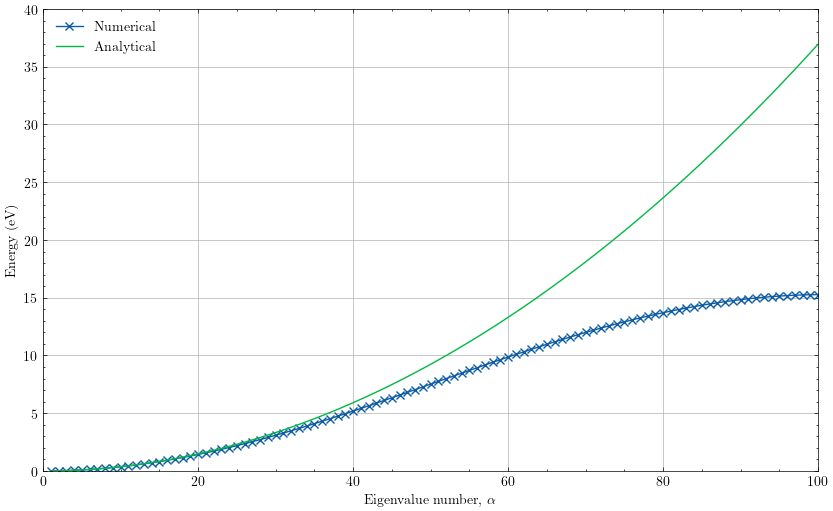
\includegraphics[scale=0.6]{discrete_PIB.png}
\caption{\textit{Numerical evaluation yields 100 eigenvalues that follow the analytical result well for low energies but deviate at higher energies because the wavefunctions oscillate too rapidly.}}\label{discrete_PIB}
\end{figure}

\vspace{1cm}

The process of discretization did not yield an accurate analytical answer in this case since the setup itself is intrinsically continuous. However, for the problems we are interested in, this process yields fairly accurate solutions since the periodic nature of the lattice then facilitates its description as a discretized system. 

\clearpage

\subsection{Toy Examples}

Consider a toy one-dimensional solid composed of $N$ atoms, separated by a distance $a$. Assuming one orbital per atom and periodic boundary condition, the $N\times N$ Hamiltonian matrix can be written as follows:

\begin{equation}
H =
\begin{matrix}
     & \ket{1} & \ket{2} & \ldots & \ket{N-1} & \ket{N} \\
    \ket{1} & E_0 & E_{ss} & \ldots & 0 & E_{ss} \\
    \ket{2} & E_{ss} & E_0 & \ldots & 0 & 0 \\
    \vdots  &  &  &  &  &  \\
    \ket{N-1} & 0 & 0 & \ldots & E_0 & E_{ss} \\
    \ket{N} & E_{ss} & 0 & \ldots & E_{ss} & E_0 \\
\end{matrix}   
\end{equation}

The off-diagonal elements at the top-right and the bottom-left are to account for the fact that we are applying the \textit{periodic boundary condition}. The set of equations (all identical in form) that we obtain by applying $[H]\psi = E\psi$ can be written as ($n = 1, 2,\ldots N$)
\begin{equation*} \label{toy_prob}
    E\psi_{n} = E_0\psi_{n} + E_{ss}\psi_{n-1} + E_{ss}\psi_{n+1}
\end{equation*}

This set of equations can be solved analytically by the ansatz (via Bloch's Theorem):
\begin{equation*} 
    \psi_{n} = \psi_0 e^{ikna} \quad \text{where} \quad ka = n2\pi/N
\end{equation*}

Substituting the ansatz into \ref{toy_prob}, we obtain
\begin{equation}
    E = E_0 + 2E_{ss}cos(ka)
\end{equation}

It would seem logically inconsistent that while we started out with a $N \times N$ Hamiltonian and were expected to find $N$ discrete eigenvalues, we have instead found a continuous, periodic function apparently implying that we have infinitely many possible eigenvalues. However, there is something more subtle at work here - due to the discrete nature of the lattice, values of $ka$ that differ by $2\pi$ represent identical states, which can be verified by considering the ansatz ($k^{'} = k + 2\pi/a$):

\begin{equation*}
\begin{aligned}
    \psi_{n}^{'} &= \psi_{0}e^{ik^{'}na} = \psi_{0}e^{ikna}e^{in2\pi} \\
    \psi_{n}^{'} &= \psi_{0}e^{ikna} = \psi_{n}
\end{aligned}
\end{equation*}

Since only the values of $ka$ within a range of $2\pi$ yield independent solutions, in principle, we could take any range of size $2\pi$, and it would be physically acceptable. It is common to restrict $ka$ to the range $-\pi < ka < \pi$, otherwise known as the first Brillouin zone. Note that while we have now limited the possible eigenvalues within the first BZ, the continuous function seemingly implies that there are still infinitely many eigenvalues within the zone itself. This issue can be resolved by taking into consideration the periodic boundary condition applied to the Hamiltonian initially: $\psi_{0} = \psi_{N}$. This implies

\begin{equation*}
\begin{aligned}
    \psi_{0} &= \psi_{N} = \psi_{0}e^{ikNa} \\
    ka &= \frac{2\pi}{N}\nu
\end{aligned}  
\end{equation*}

where $\nu \in Z$. Thus, we end up with $N$ discrete energy eigenvalues, all bound within the first Brillouin zone, as intended from physical intuition.

\vspace{1cm}

\begin{figure}[h]
\centering
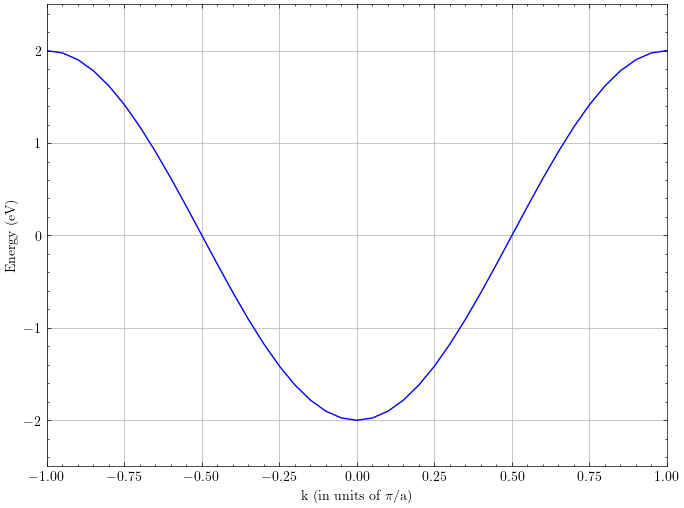
\includegraphics[scale=0.6]{1D_chain.png}
\caption{\textit{Bandstructure for a one-dimensional solid with $E_0 = 0$ and $E_{ss} = -1$.}}
\end{figure}

\vspace{1cm}

